\usetikzlibrary{arrows.meta}
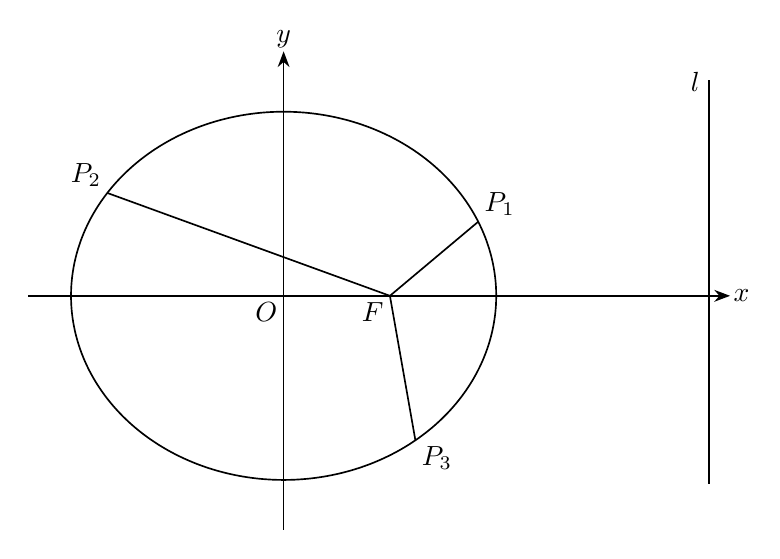
\begin{tikzpicture}[x=0.45cm,y=0.45cm,line width=.6pt,>=Stealth,font=\normalsize]
  \def\ellA{6}
  \def\ellB{5.196152423}
  \def\ellC{3}
  \coordinate (O) at (0,0);
  \coordinate (F) at (3,0);
  \coordinate (Pone) at (5.492512,2.091466);
  \coordinate (Ptwo) at (-4.976209,2.903103);
  \coordinate (Pthree) at (3.718991,-4.077601);
  \draw[->] (-7.2,0) -- (12.6,0) node[right,inner sep=1pt] {$x$};
  \draw[->] (0,-6.6) -- (0,6.9) node[above,inner sep=1pt] {$y$};
  \draw[domain=0:360,samples=241,smooth,variable=\t] plot ({\ellA*cos(\t)},{\ellB*sin(\t)});
  \draw (12,-5.3) -- (12,6.1);
  \draw (F) -- (Pone);
  \draw (F) -- (Ptwo);
  \draw (F) -- (Pthree);
  \node[below left,inner sep=2pt] at (O) {$O$};
  \node[below left,inner sep=2pt] at (F) {$F$};
  \node[above right,inner sep=2pt] at (Pone) {$P_1$};
  \node[above left,inner sep=2pt] at (Ptwo) {$P_2$};
  \node[below right,inner sep=2pt] at (Pthree) {$P_3$};
  \node[left,inner sep=3pt] at (12,6.05) {$l$};
\end{tikzpicture}
